% Encoding: UTF-8
%%%%%%%%%%%%%%%%%%%%%%%%%%%%%%%%%%%%%%%%%%%%%%%%%%%%%%%%%%%%%%%%%%%%%%%%%%%%%%%

\documentclass[xcolor=pdftex,dvipsnames,table]{beamer}
\setbeamertemplate{navigation symbols}{}%remove navigation symbols
%%%%%%%%%%%%%%%%%%%%%%%%%%%%%%%%%%%%%%%%%%%%%%%%%%%%%%%%%%%%%%%%%%%%%%%%%%%%%%%

% Language settings
% IMPORTANT: If you change the language settings, make sure to run
% cleantex prior to any latex/pdflatex to remove all .aux files, else
% latex might fail!
\usepackage[english]{babel}
%\usepackage[german]{babel}
\usecolortheme{rose}
\usecolortheme{beaver}
\useinnertheme[shadow]{rounded}
\usecolortheme{dolphin}
%\usepackage{graphicx}
\usepackage[utf8]{inputenc}
%\usepackage{mathptmx}

\usepackage{setspace}
\usepackage{color}
\usepackage{listings}
	
	
%%%%%%%%%%%%%%%%%%%%%%%%%%%%%%%%%%%%%%%%%%%%%%%%%%%%%%%%%%%%%%%%%%%%%%%%%%%%%%%

% IMPORTANT/TODO: currently only PDF graphic files should be used, PNG
% or JPEG may harm the Adobe Reader colour palette and result in
% strange display colours.
%\DeclareGraphicsExtensions{.pdf}


%%%%%%%%%%%%%%%%%%%%%%%%%%%%%%%%%%%%%%%%%%%%%%%%%%%%%%%%%%%%%%%%%%%%%%%%%%%%%%%
%% Presentation main settings
%%%%%%%%%%%%%%%%%%%%%%%%%%%%%%%%%%%%%%%%%%%%%%%%%%%%%%%%%%%%%%%%%%%%%%%%%%%%%%%

\title{Systemnahe Informatik}
\subtitle{Übungsgruppe Xeon Phi}
\author{Dominik Walter}
\date{Sommersemester 2018}


%%%%%%%%%%%%%%%%%%%%%%%%%%%%%%%%%%%%%%%%%%%%%%%%%%%%%%%%%%%%%%%%%%

\begin{document}

\section*{Titlepage}
\begin{frame}
  \frametitle{\ }
  \titlepage
\end{frame}

%%%%%%%%%%%%%%%%%%%%%%%%%%%%%%%%%%%%%%%%%%%%%%%%%%%%%%%%%%%%%%%%%%%%%%%%%%%%%%%

\begin{frame}[fragile]
	\frametitle{Zugriffsmuster auf eine Matrix}
	\begin{block}{Zeilenweises Iterieren}
		\begin{lstlisting}	
for (int y = 0; y < size; y++) {
	for (int x = 0; x < size; x++) {
		matrix[y * size + x] = x * y;
	}
}
		\end{lstlisting}
	\end{block}

	\begin{block}{Spaltenweises Iterieren}
		\begin{lstlisting}		
for (int x = 0; x < size; x++) {
	for (int y = 0; y < size; y++) {
		matrix[y * size + x] = x * y;
	}
}
		\end{lstlisting}
	\end{block}	
\end{frame}

\begin{frame}
	\frametitle{Zugriffsmuster auf eine Matrix}
	
	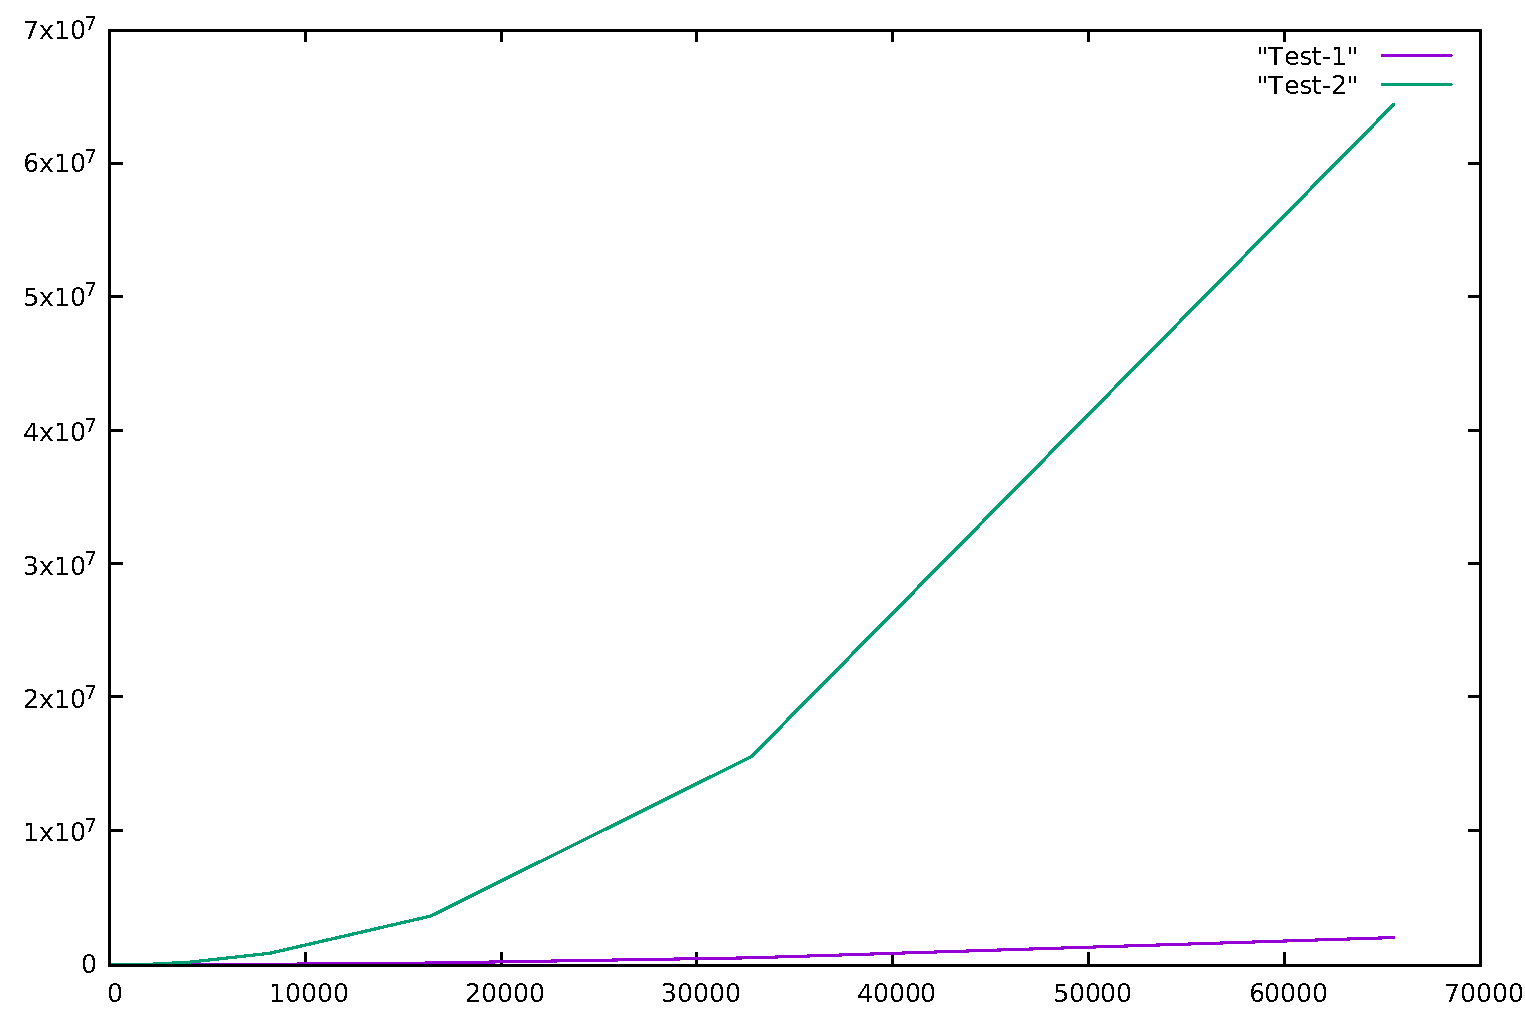
\includegraphics[width=10cm]{matrix_result.pdf}
\end{frame}

\begin{frame}
	\frametitle{Zugriffsmuster auf eine Matrix}
	\begin{columns}
		\begin{column}{0.5\textwidth}
			8 Cache-Lines mit jeweils 8 Byte\\
			\begin{tabular}{|c|c|c|c|}
				\hline
				(0, 0) & (1, 0) & (2, 0) & (3, 0) \\
				0x00 & 0x04 & 0x08 & 0x0C \\
				\hline
				\multicolumn{2}{|c|}{Tag: 0x0,0} &
				\multicolumn{2}{c|}{Tag: 0x0,1} \\
				\hline
				\hline
				(0, 1) & (1, 1) & (2, 1) & (3, 1) \\
				0x10 & 0x14 & 0x18 & 0x1C \\
				\hline
				\multicolumn{2}{|c|}{Tag: 0x1,0} &
				\multicolumn{2}{c|}{Tag: 0x1,1} \\
				\hline
				\hline
				(0, 2) & (1, 2) & (2, 2) & (3, 2) \\
				0x20 & 0x24 & 0x28 & 0x28 \\
				\hline
				\multicolumn{2}{|c|}{Tag: 0x2,0} &
				\multicolumn{2}{c|}{Tag: 0x2,1} \\
				\hline
				\hline
				(0, 3) & (1, 3) & (2, 3) & (3, 3) \\
				0x30 & 0x34 & 0x38 & 0x3c \\
				\hline
				\multicolumn{2}{|c|}{Tag: 0x3,0} &
				\multicolumn{2}{c|}{Tag: 0x3,1} \\
				\hline
			\end{tabular}
		\end{column}
		\begin{column}{0.5\textwidth}
			\begin{block}{Zeilenweise}
				0x0,0 $\rightarrow$ 0x0,0 $\rightarrow$ 0x0,1 $\rightarrow$ 0x0,1 0x1,0 $\rightarrow$ 0x1,0 $\rightarrow$ 0x1,1 $\rightarrow$ 0x1,1  0x2,0 $\rightarrow$ 0x2,0 $\rightarrow$ 0x2,1 $\rightarrow$ 0x2,1  0x3,0 $\rightarrow$ 0x3,0 $\rightarrow$ 0x3,1 $\rightarrow$ 0x3,1
			\end{block}
			\begin{block}{Spaltenweise}
				0x0,0 $\rightarrow$ 0x1,0 $\rightarrow$ 0x2,0 $\rightarrow$ 0x3,0 0x0,0 $\rightarrow$ 0x1,0 $\rightarrow$ 0x2,0 $\rightarrow$ 0x3,0  0x0,1 $\rightarrow$ 0x1,1 $\rightarrow$ 0x2,1 $\rightarrow$ 0x3,1  0x0,1 $\rightarrow$ 0x1,1 $\rightarrow$ 0x2,1 $\rightarrow$ 0x3,1
			\end{block}
		\end{column}
	\end{columns}


	
\end{frame}

\begin{frame}[fragile]
	\frametitle{std::vector vs. std::list}
	\begin{block}{std::vector}
	\begin{lstlisting}	
std::vector<int> vector;
for (auto x: vector) {
	result += x;
}
	\end{lstlisting}
\end{block}	
\begin{block}{std::list}	
	\begin{lstlisting}	
std::list<int> list;
for (auto x: list) {
	result += x;
}
	\end{lstlisting}
\end{block}
\end{frame}

\begin{frame}[fragile]
	\frametitle{Array vs. Liste}
	\begin{columns}
		\begin{column}{0.5\textwidth}
\begin{block}{Array}
\begin{lstlisting}	
start:
beq     t0, a2, end

lw      t3, 0(a1)
add     a0, a0, t3

add     a1, a1, 4
add     t0, t0, 1
j start
end:
\end{lstlisting}
\end{block}
		\end{column}
		\begin{column}{0.5\textwidth}
			\begin{block}{Liste}
\begin{lstlisting}	
# struct node {
#       node* next;
#       int data;
# }

start:
beq     a1, zero, end

lw      t0, 4(a1)
add     a0, a0, t0

lw      a1, 0(a1)
j start
end:
\end{lstlisting}
\end{block}
		\end{column}
	\end{columns}
\end{frame}

\begin{frame}
	\frametitle{std::vector vs. std::list}
	
	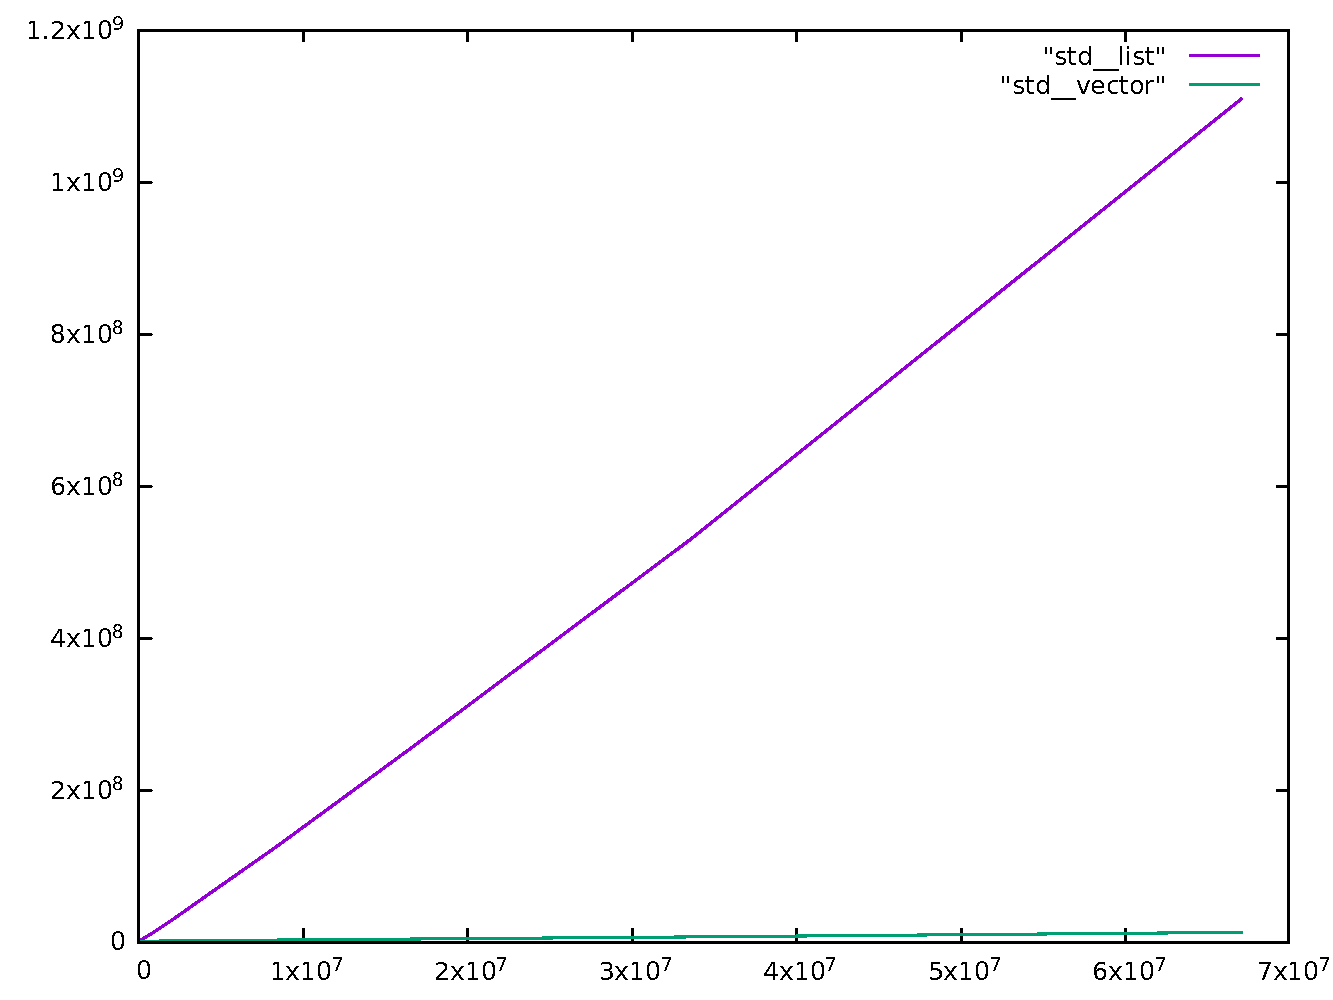
\includegraphics[width=10cm]{vector_list_result.pdf}
\end{frame}

\begin{frame}
	\frametitle{Zugriffsmuster eines Arrays}
			2 Cache-Lines mit jeweils 8 Byte\\
			\begin{tabular}{|c|c|c|c|c|c|c|c|c|c|c|c|c|c|c|c|}
				\hline
				0 & 1 & 2 & 3 & 4 & 5 & 6 & 7 & 8 & 9 & 10 & 11 & 12 & 13 & 14 & 15 \\
				\hline
				C & a & c & h & e & s & \  & s & i & n & d & \  & t & o & l & l \\
				\hline
				\multicolumn{8}{|c|}{Tag: 0x0,0} &
				\multicolumn{8}{c|}{Tag: 0x0,1} \\
				\hline
			\end{tabular}
			\begin{block}{Zugriffsmuster:}
			\small{
			0x0,0 $\rightarrow$ 0x0,0 $\rightarrow$ 0x0,0 $\rightarrow$ 0x0,0 $\rightarrow$ 0x0,0 $\rightarrow$ 0x0,0 $\rightarrow$ 0x0,0 $\rightarrow$ 0x0,0
			
			 $\rightarrow$ 0x0,1 $\rightarrow$ 0x0,1 $\rightarrow$ 0x0,1 $\rightarrow$ 0x0,1 $\rightarrow$ 0x0,1 $\rightarrow$ 0x0,1 $\rightarrow$ 0x0,1 $\rightarrow$ 0x0,1
			}
			\end{block}
\end{frame}

\begin{frame}
	\frametitle{Zugriffsmuster einer Liste}
	Hinweis: Hier nur 8 Bit pro Pointer!
	\begin{tabular}{|c|c|c|c|c|c|c|c|c|c|c|c|c|c|c|c|}
		\hline
		\color{red}{18} & \color{red}{C} & q & s & \color{red}{22} & \color{red}{n} & x & d & \color{red}{26} & \color{red}{s} & e & f  & r & b & c & y \\
		\hline
		\multicolumn{8}{|c|}{Tag: 0x0,0} &
		\multicolumn{8}{c|}{Tag: 0x0,1} \\
		\hline
		\hline
		i & k & \color{red}{36} & \color{red}{a} & g & q & \color{red}{40} & \color{red}{d} & v & m & \color{red}{44} & \color{red}{\_}  & t & o & h & w \\
		\hline
		\multicolumn{8}{|c|}{Tag: 0x1,0} &
		\multicolumn{8}{c|}{Tag: 0x1,1} \\
		\hline
		\hline
		\color{red}{50} & \color{red}{l} & c & h & \color{red}{54} & \color{red}{c} & \  & s & \color{red}{58} & \color{red}{\_} & d & k & \color{red}{62} & \color{red}{s} & o & l \\
		\hline
		\multicolumn{8}{|c|}{Tag: 0x2,0} &
		\multicolumn{8}{c|}{Tag: 0x2,1} \\
		\hline
		\hline
		f & a & \color{red}{0} & \color{red}{l} & e & s & \color{red}{72} & \color{red}{h} & i & n & \color{red}{76} & \color{red}{t}  & h & q & \color{red}{4} & \color{red}{i} \\
		\hline
		\multicolumn{8}{|c|}{Tag: 0x3,0} &
		\multicolumn{8}{c|}{Tag: 0x3,1} \\
		\hline
		\hline
		b & g & z & u & j & k & d & w & \color{red}{8} & \color{red}{e} & c & t & \color{red}{32} & \color{red}{o} & a & p \\
		\hline
		\multicolumn{8}{|c|}{Tag: 0x4,0} &
		\multicolumn{8}{c|}{Tag: 0x4,1} \\
		\hline
	\end{tabular}
	\begin{block}{Zugriffsmuster: (jeweils 2x)}
	\small{
		0x0,0 $\rightarrow$ 0x1,0 $\rightarrow$ 0x2,0 $\rightarrow$ 0x3,0 $\rightarrow$ 0x4,1 $\rightarrow$ 0x0,1 $\rightarrow$ 0x1,1 $\rightarrow$ 0x2,1
		
		$\rightarrow$ 0x3,1 $\rightarrow$ 0x0,0 $\rightarrow$ 0x1,0 $\rightarrow$ 0x2,1 $\rightarrow$ 0x3,1 $\rightarrow$ 0x4,1 $\rightarrow$ 0x2,0 $\rightarrow$ 0x3,0
	}
	\end{block}
\end{frame}

\end{document}

%%%%%%%%%%%%%%%%%%%%%%%%%%%%%%%%%%%%%%%%%%%%%%%%%%%%%%%%%%%%%%%%%%%%%%%%%%%%%%%
